\section{Personal Objective---Communication Skills}
\subsection{Objective}
\emph{Use a range of communication skills}. 
For this objective, I've chosen to focus on a weak point of mine: presentations. There weren't many opportunities for me to develop my presentation skills throughout the year, but when I've had the chance, I've made sure to pay attention to what went well and what I can improve \parencite[][p. 5, entry 23/04/2021]{scanlan_2021}.

\begin{figure}[ht]
    \caption{\small{\emph{Feedback received on sprint review.}}}
    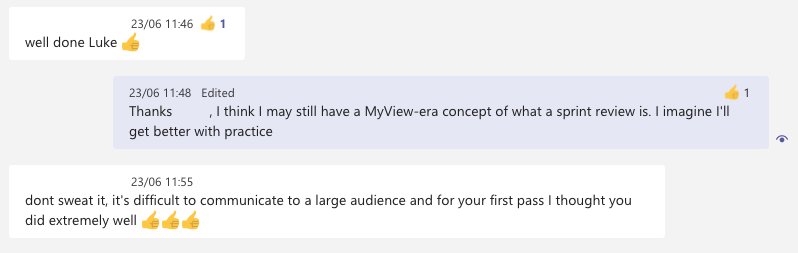
\includegraphics[width=\textwidth]{sprint review feedback}
    \label{fig:revfeedback}
\end{figure}

\paragraph{Learning}
\begin{itemize}
    \item Talk to the product owner if the value of a task is ambiguous.
    \item Take notes on what teammates' good practices in sprint reviews and emulate them.
    \item Feelings aren't facts, don't let your negative thoughts win.
    \item Embrace being uncomfortable with presenting until it becomes comfortable.
\end{itemize}
